
\subsection{Plan del proyecto}

\subsection{Estimación de recursos}

\subsubsection{Materiales}

\begin{table}[H]
 \begin{center}
  \begin{tabular}{llll}
	\textbf{ID Unidad} & \textbf{Descripción} & \textbf{Unidad de medición} & \textbf{Nº de unidades} \\
	HW1 & Ordenador de tipo PC & unidad & 1
  \end{tabular}
  \caption{Recursos hardware}
 \end{center}
\end{table}

\begin{table}[H]
 \begin{center}
  \begin{tabular}{llll}
	\textbf{ID Unidad} & \textbf{Descripción} & \textbf{Unidad de medición} & \textbf{Nº de unidades} \\
	SW1 & S.O. GNU/Linux & unidad & 1 \\
	SW2 & Interprete de Python & unidad & 1 \\
	SW3 & Entorno de desarrollo Eclipse & unidad & 1 
  \end{tabular}
  \caption{Recursos software}
 \end{center}
\end{table}

\subsubsection{Personales}

\begin{table}[H]
 \begin{center}
  \begin{tabular}{llll}
	\textbf{ID Unidad} & \textbf{Descripción} & \textbf{Unidad de medición} & \textbf{Nº de unidades} \\
	HU1 & Análisis y diseño & horas & 200 \\
	HU2 & Desarrollo del software & horas & 550 \\
	HU3 & Dirección técnica & horas & 70 
  \end{tabular}
  \caption{Recursos personales}
 \end{center}
\end{table}

\subsubsection{Etapas del proyecto}

El desarrollo del proyecto ha quedado delimitado en varias etapas claramente
delimitadas.

Las principales etapas, también recogidas en el gráfico de gantt de la 
figura~\ref{fig:gantt}, se enumeran en la siguiente tabla:


\begin{table}[H]
 \begin{center}
  \begin{tabular}{llll}
	\textbf{WBS} & \textbf{Tarea} & \textbf{Inicio} & \textbf{Fin} \\
	\textbf{1}   & Especificación de requisitos y estudio de viabilidad & 26/09/2005 & 09/01/2006 \\
	\textbf{2}   & Análisis y Diseño & 09/01/2006 & 15/02/2006 \\
	\textbf{3}   & Desarrollo Software & 19/01/2006 & 21/11/2006 \\
	\textbf{3.1} & Desarrollo del core de SWAML & 19/01/2006 & 18/08/2006 \\	
	\textbf{3.2} & Desarrollo de Buxon & 18/08/2006 & 01/11/2006 \\
	\textbf{3.3} & Desarrollo de herramientas complementarias & 07/09/2006 & 21/11/2006 \\	
	\textbf{4}   & Elaboración de la documentación & 01/06/2006 & 30/11/2006 \\	
	\textbf{5}   & Dirección & 26/09/2005 & 01/12/2006
  \end{tabular}
  \caption{Reparto de tareas}
 \end{center}
\end{table}

\begin{figure}[p]
 	\centering
	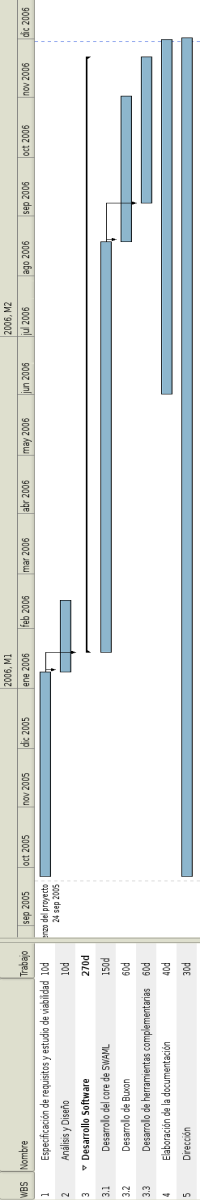
\includegraphics[width=5cm]{images/gantt.png}
	\caption{Planificación general del proyecto}
	\label{fig:gantt}
\end{figure}

%FIXME: conseguir exportarlo con los periodos a más detalle

\subsection{Presupuesto}

\subsubsection{Tabla de precios}

FIXME: conseguir la tabla de precios oficial

\begin{table}[H]
 \begin{center}
  \begin{tabular}{llll}
	\textbf{ID Unidad} & \textbf{Descripción} & \textbf{Unidad de medición} & \textbf{Precio} \\
	HW1 & Ordenador de tipo PC & \euro/ud & 1.190 \\
	SW1 & S.O. GNU/Linux & \euro/ud & 0 \\
	SW2 & Interprete de Python & \euro/ud & 0 \\
	SW3 & Entorno de desarrollo Eclipse & \euro/ud & 0 \\
	HU1 & Análisis y diseño & \euro/h & 57,01 \\
	HU2 & Desarrollo del software & \euro/h & 36,51 \\
	HU3 & Dirección técnica & \euro/h & 71,85 
  \end{tabular}
  \caption{Tabla de precios}
 \end{center}
\end{table}

\subsubsection{Presupuestos parciales}

\begin{table}[H]
 \begin{center}
  \begin{tabular}{lll}
	\textbf{ID Unidad} & \textbf{Descripción} & \textbf{Importe} \\
	HW1 & Ordenador de tipo PC & 1.190,00 \euro
  \end{tabular}
  \caption{Presupuesto parcial de recursos hardware}
 \end{center}
\end{table}

\begin{table}[H]
 \begin{center}
  \begin{tabular}{lll}
	\textbf{ID Unidad} & \textbf{Descripción} & \textbf{Importe} \\
	SW1 & S.O. GNU/Linux & 0,00 \euro \\
	SW2 & Interprete de Python & 0,00 \euro \\
	SW3 & Entorno de desarrollo Eclipse & 0,00 \euro
  \end{tabular}
  \caption{Presupuesto parcial de recursos software}
 \end{center}
\end{table}

\begin{table}[H]
 \begin{center}
  \begin{tabular}{lll}
	\textbf{ID Unidad} & \textbf{Descripción} & \textbf{Importe} \\
	HU1 & Análisis y diseño & 11.402,00 \euro \\
	HU2 & Desarrollo del software & 20.080,50 \euro \\
	HU3 & Dirección técnica & 5.010,60 \euro 
  \end{tabular}
  \caption{Presupuesto parcial de recursos personales}
 \end{center}
\end{table}

\subsubsection{Presupuesto final}

%FIXME: retocar cuando tenga la tabla de precios oficial

\begin{table}[H]
 \begin{center}
  \begin{tabular}{ll}
	\textbf{Descripción} & \textbf{Importe} \\
	Recursos hardware & 1.190,00 \euro \\
	Recursos software & 0,00 \euro \\
	Recursos personales & 36.493,10 \euro \\
	\textbf{SUBTOTAL} & \textbf{37.683,10 \euro} \\
	Beneficio industrial (6\%) & 2.260,99 \euro \\
	Costes generales (15\%) & 5.652,47 \euro \\
	Suma de gastos y beneficios & 45.596,55 \euro \\
	I.V.A. (16\%) & 7.295,49 \euro \\
	\textbf{TOTAL} & \textbf{52.892 \euro}
  \end{tabular}
  \caption{Presupuesto final}
 \end{center}
\end{table}
